\documentclass[11pt]{beamer}

%my colours


\usetheme{metropolis}
\metroset{everytitleformat = regular,progressbar=foot} %settings
\mode<presentation>
%\usecolortheme{dove} %dove
% albatross, beaver, beetle, crane, default, dolphin, dove, orchid, rose, seagull, seahorse, whale, wolverine
%dont use  fly, lily,
%http://mirror.ox.ac.uk/sites/ctan.org/macros/latex/contrib/beamer/doc/beameruserguide.pdf
\setbeamercolor{title separator}{fg = UniBlue}
\setbeamercolor{frametitle}{fg = deepBlue, bg=aBlue!70}

\usepackage{booktabs}
\usepackage[scale=2]{ccicons}

\usepackage{pgfplots}
\usepgfplotslibrary{dateplot}


%coords are in relation to lower right corner
%\logo{\pgfputat{\pgfxy(0,6}{\pgfbox[right,top]{
\includegraphics[width=2.5cm]{logo.png}}}}

\usepackage{tikz}
\addtobeamertemplate{frametitle}{}{%
\begin{tikzpicture}[remember picture,overlay]
\node[anchor=north east,yshift=2pt] at (current page.north east) {
\includegraphics[height=0.8cm]{./../logo.png}};
\end{tikzpicture}}

%My std preamble for the docs
%\selectlanguage{british}%
\usepackage[british]{babel}
\usepackage{microtype} %better text
\IfFileExists{lmodern.sty}{\usepackage{lmodern}}{} %type 1 vector font
%
\usepackage{lettrine}
\usepackage{listings} %Add list support
\usepackage{colortbl} %colors in TABLES
%\usepackage{tikz,amsmath, amssymb,bm,color}
\usepackage{nicefrac}
\usepackage{lastpage} %get last page

%COLORS
\usepackage{color}
\definecolor{lightgray}{gray}{0.8} %for colortbl
\definecolor{UniBlue}{RGB}{83,121,170}
\definecolor{deepBlue}{HTML}{000066}
\definecolor{blueBgd}{HTML}{99C8FF}
\definecolor{aBlue}{HTML}{1879F7}

%%%%%%%%%%%%%%%%%%%%%%%%%%%%%%%%%%%%%%%%%%%%%%%%%%%%%%%%%%%%%%%%%%
%FOOTNOTES
%nice look after http://www.dedoimedo.com


%%%%%%%%%%%%%%%%%%%%%%%%%%%%%%%%%%%%%%%%%%%%%%%%%%%%%%%%%%%%%%%%%%%
%TABLE SETTINGS
\usepackage{colortbl} %colors in table
\usepackage{rotating} %rotatins within tables
\usepackage{multirow}
\renewcommand{\arraystretch}{1.2} %add padding/spacing
%\usepackage{adjustbox}%rotating and fitting into page
%

\usepackage{booktabs} % To thicken table lines
%define thickness of table lines
\let\mytoprule\toprule
\renewcommand{\toprule}{\mytoprule[0.20em]}
\let\mytoprule\bottomrule
\renewcommand{\bottomrule}{\mytoprule[0.20em]}
\let\mytoprule\midrule
\renewcommand{\midrule}{\mytoprule[0.08em]}

\usepackage{spreadtab} % for simple calculations

%vertically and horizontally centered multicolumn cells with a fixed width. M{width}
%\newcolumntype{M}[1]{>{\centering\hspace{0pt}}m{#1}}
% each spanned cell has the same width. S{width of multicolumn cell}{number of spanned columns}
%\newcolumntype{S}[2]{>{\centering\hspace{0pt}}m{(#1+(2\tabcolsep+\arrayrulewidth)*(1-#2))/#2}}

%%%%%%%%%%%%%%%%%%%%%%%%%%%%%%%%%%%%%%%%%%%%%%%%%%%%%%%%%%%%%%%%%%%
%TikZ
\usepackage{tikz}

\colorlet{red}{red!50}
\colorlet{green}{green!50}
\colorlet{blue}{blue!50}
\definecolor{yellow}{HTML}{FFFF00}
\colorlet{yellow}{yellow!50}
\definecolor{fiolet}{HTML}{7030A0}
\colorlet{fiolet}{fiolet!50}
\colorlet{bgd_main}{black!50}
\colorlet{bgd}{bgd_main!75}
\colorlet{bgd2}{bgd_main!50}
\colorlet{bgd3}{bgd_main!25}
\colorlet{bgd4}{bgd_main!15}

\usetikzlibrary{shapes,arrows,calc,positioning}

%%%%%%%%%%%%%%%%%%%%%%%%%%%%%%%%%%%%%%%%%%%%%%%%%%%%%%%%%%%%%%%%%%%
% Footnotes in Figs
%\rule[raise-height]{width}{thickness}
\newcommand*{\FigFootnote}[1]{
\noindent \begin{flushleft}
\rule[0.2ex]{0.4\columnwidth}{0.5pt}
\par
\footnotesize
#1
\footnotesize
\end{flushleft}
}

%%%%%%%%%%%%%%%%%%%%%%%%%%%%%%%%%%%%%%%%%%%%%%%%%%%%%%%%%%%%%%%%%%%
%MATH, number display
%need to install siunitx, l3kernel,l3packages
\usepackage{siunitx} %this is for units display

\sisetup{per-mode=fraction, tight-spacing = true , fraction-function = \nicefrac, quotient-mode = fraction}% %nicefrac \tfrac
\sisetup{inter-unit-product = \ensuremath { { } \cdot { } } , exponent-product = \cdot }%
\sisetup{input-product=x , output-quotient =  \ensuremath { { } \times{}}} %for 1x2x3
%number grouping(3), std==true %\sisetup{group-digits = decimal} 
\sisetup{group-minimum-digits = 4} %start grouping from 4 digits, in 3 no groups
\sisetup{range-units = single,range-phrase = \,--\,} %2-3C not 2C-3C %, range-phrase = --
\sisetup{separate-uncertainty=true} %2+-1 not 2(1)
\sisetup{prefixes-as-symbols=true } % , scientific-notation = engineering false for 10^-9 ect ect , exp in multiple of 3
\sisetup{range-phrase = \,-\, } % , refo of ranges
%\sisetup{zero-decimal-to-integer, round-mode = places,round-precision = 3}
%\sisetup{add-arc-degree-zero=true , add-arc-minute-zero=true ,add-arc-second-zero=true} %for angle settings

%This is to auto convert ns,ms,us to 10^-xx s
\DeclareSIUnit[scientific-notation = engineering, prefixes-as-symbols=false]{\psec}{\pico\second}
\DeclareSIUnit[scientific-notation = engineering, prefixes-as-symbols=false]{\nsec}{\nano\second} 
\DeclareSIUnit[scientific-notation = engineering, prefixes-as-symbols=false]{\usec}{\micro\second}
\DeclareSIUnit[scientific-notation = engineering, prefixes-as-symbols=false]{\msec}{\milli\second} 

%...AND SOME UNITS
\DeclareSIUnit\dBm{dBm}
\DeclareSIUnit\ppm{ppm} %{\num{1e-6}}%{ppm}
\DeclareSIUnit\yr{yr} %{{361}\day}<-nice nice
\DeclareSIUnit\cy{cycle} %phase cycle
\DeclareSIUnit\epoch{epoch} %GPS/LL epoch
\DeclareSIUnit\inch{"} %inch 
\DeclareSIUnit\wk{week} %week
\DeclareSIUnit\hr{hrs} %hours
\DeclareSIUnit\min{minute} %hours
\DeclareSIUnit\mile{mi}
\DeclareSIUnit\Mcps{Mcps}
\DeclareSIUnit\bit{bit}
\DeclareSIUnit\chip{chip length}
%Other units
\newcommand*{\GBP}[1]{$\SI{#1}[\textsterling]{}$}


%%%%%SHORTHANDS (Standard Sentences)
%\newcommand*{\Myrange}[3]{$\textrm{\SIrange{#1}{#2}{#3}}$}


%how much work per week
\newcommand*{\wkWrk}[1]{$\SI{#1}{\hr\per\wk}$}

%references
\newcommand*{\tabref}[1]{shown in table \ref{#1} on page \pageref{#1}\xspace}
\newcommand*{\vref}[1]{\ref{#1} on page \pageref{#1}\xspace}


%\renewcommand{\baselinestretch}{1.2} %line spacing
%{\setstretch{1.0}\color{blue} text bla bla } for section strech
\renewcommand{\footnotesize}{\scriptsize}
%\usepackage[demo]{graphicx}
\usepackage[font={small,it}]{caption}
%\usepackage{subcaption}

%%%%%%%%%%%%%%%%%%%%%%%%%%%%%%%%%%%%%%%%%%%%%%%%%%%%%%%%%%%%%%%%%%%%%%%%%%%%%%

\title[RR]{Reproducible Research}
\subtitle{and why to do it...}
\author{Lukasz K Bonenberg}
\institute{NGI}

\date{\today}
\titlegraphic{\hfill
\includegraphics[height=1.3cm]{./../bigLogo.png}}

\begin{document}

\maketitle

\begin{frame}{Table of Contents\thisDocRef}

  \setbeamertemplate{section in toc}[sections numbered]
  \tableofcontents[hideallsubsections]
\end{frame}


%%%%%%%%%%%%%%%%%%%%%%%%%%%%%%%%%%%%%%%%%%%%%%%%%%%%%%%%%%%%%%%%%%%%%%%%%%%%%%%%%%%%%%%%
\section{Introduction}


\begin{frame}{}%{Daily repetition}

	\begin{exampleblock}{}
\begin{itemize}
	\item report\_01.doc
	\item report\_02.doc
	\item report\_03\_revByJim.doc
	\item report\_04\_changes.doc
	\item report\_05\_final.doc
	\item report\_05\_finalFinal.doc
	\item report\_05\_finalFinal\_FINAL.doc
	\item report\_05\_finalFinal\_FINAL\_send.doc

\end{itemize}
	\end{exampleblock}

\end{frame}

\begin{frame}{Entropy}%{Daily repetition}

\centering
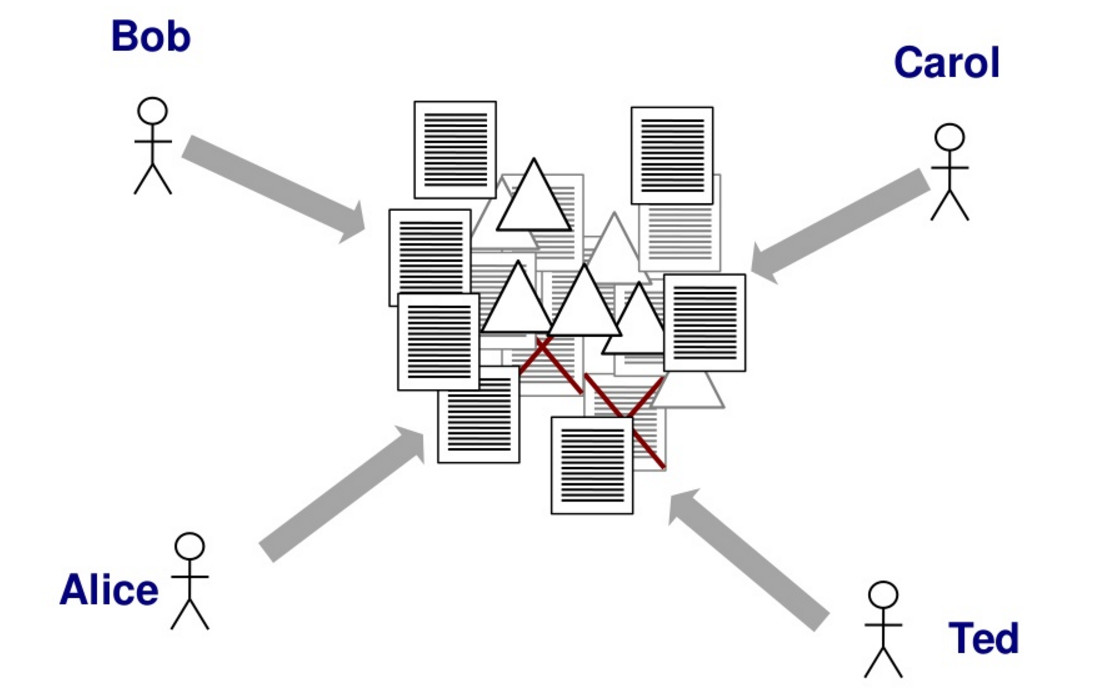
\includegraphics[width=\textwidth]{pic/disaster.jpg}\footnote{\url{http://www.slideshare.net/jomikr/quick-introduction-to-git}}

\end{frame}



%%%%%%%%%%%%%%%%%%%%%%%%%%%%%%%%%%%%%%%%%%%%%%%%%%%%%%%%%%%%%%%%%%%%%%%%%%%%%%%%%%%%%%%%
\section{git - Version Control}

\begin{frame}{Control the time}%{Daily repetition}
	\centering
	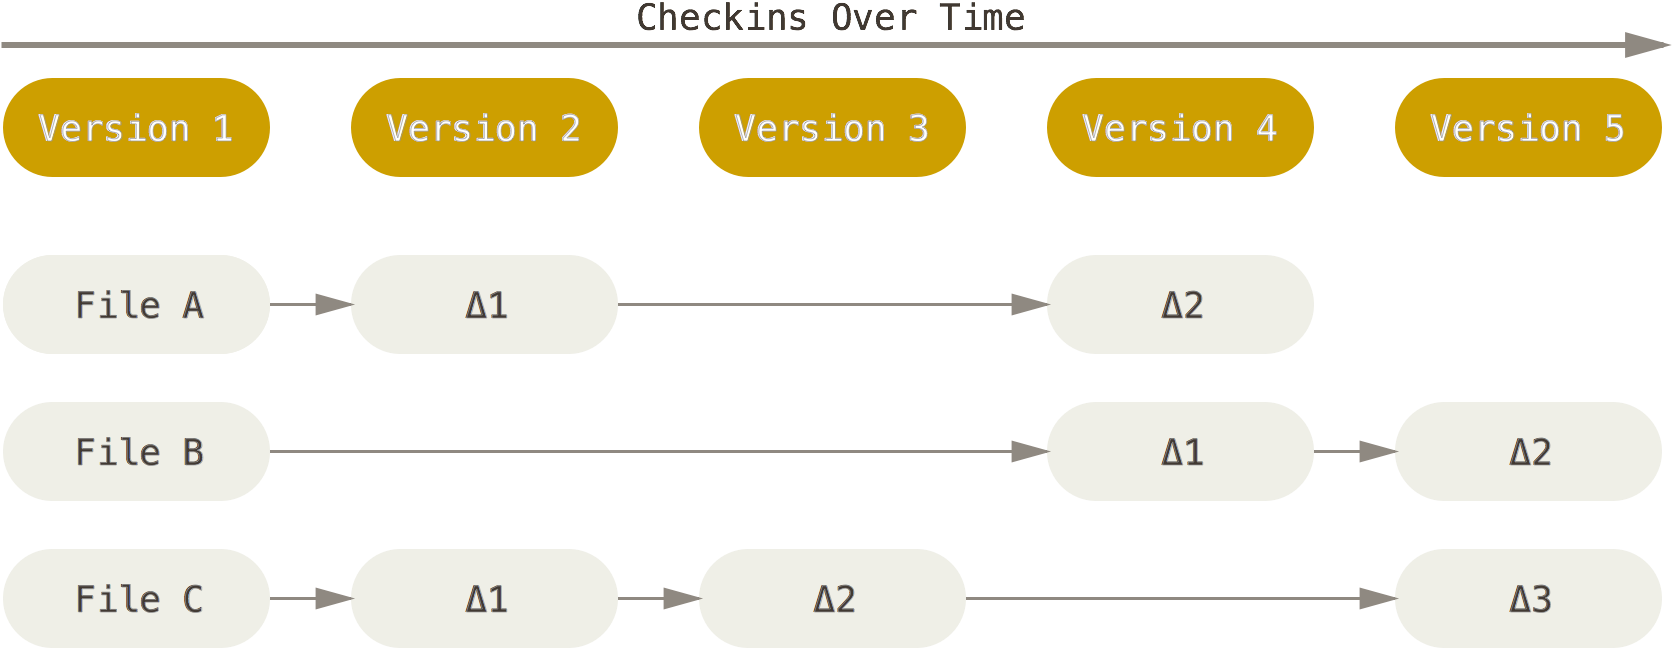
\includegraphics[width=\textwidth]{pic/git01.png}\footnote{\url{https://git-scm.com/book/ch1-3.html}}
	%\captionof{figure}{Visualisation} %to make images on top of each other
\end{frame}


\begin{frame}{Examples}%{Daily repetition}

	\begin{itemize}
		\item \url{https://github.com/tomojitakasu/RTKLIB}
		\item \url{https://github.com/DfAC/TEQCSPEC}
	\end{itemize}

\end{frame}

\begin{frame}{Lets try it}%{Daily repetition}

	\begin{itemize}
		\item \url{http://rogerdudler.github.io/git-guide/}
		\item \url{https://try.github.io/levels/1/challenges/10}
	\end{itemize}

\end{frame}


% \begin{frame}{Summary}
% \centering
% 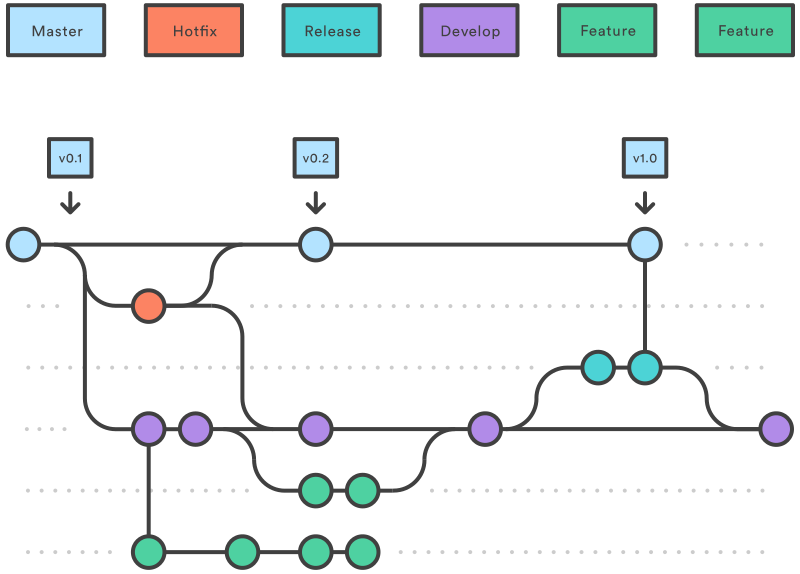
\includegraphics[height=.7\textheight]{pic/Git_flow.png}\footnote{\url{https://www.atlassian.com/git/tutorials/}}
% %\captionof{figure}{Gitflow Workflow \hfill\\\tiny{\url{https://www.atlassian.com/git/tutorials/}}}

% \end{frame}


%%%%%%%%%%%%%%%%%%%%%%%%%%%%%%%%%%%%%%%%%%%%%%%%%%%%%%%%%%%%%%%%%%%%%%%%%%%%%%%%%%%%%%%%
\section{What can we use it for?}


%\setbeamercolor{background canvas}{bg=blueBgd!60}
%\plain{Is this just for \LaTeX{} then?}
%\plain{What can we use it for?}
%\setbeamercolor{background canvas}{bg=blueBgd!0}

\begin{frame}{Team work}
\centering
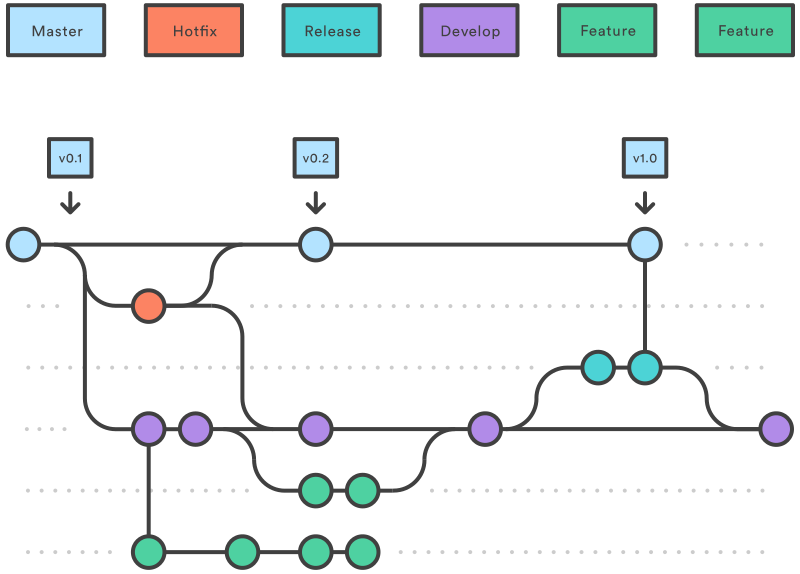
\includegraphics[height=.7\textheight]{pic/Git_flow.png} \footnote{\url{https://www.atlassian.com/git/tutorials/}}
%\captionof{figure}{Gitflow Workflow \hfill\\ \tiny{\url{https://www.atlassian.com/git/tutorials/}}} %to make images on top of each other
\end{frame}

\begin{frame}{More teaching}

\begin{itemize}
	\item \url{https://github.com/FOSS4GAcademy}
	\item \url{https://github.com/DfAC/TeachingSlides}
\end{itemize}
\end{frame}

\begin{frame}{More teaching}
Sebastien Saunier\footnote{\url{http://bit.ly/1MQLSo9}} discussed auto-marking using git.
\centering
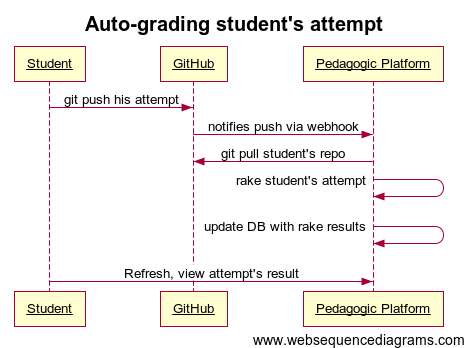
\includegraphics[height=0.7\textheight]{pic/git_teaching.png}
\end{frame}


\begin{frame}{Open Source}
\centering
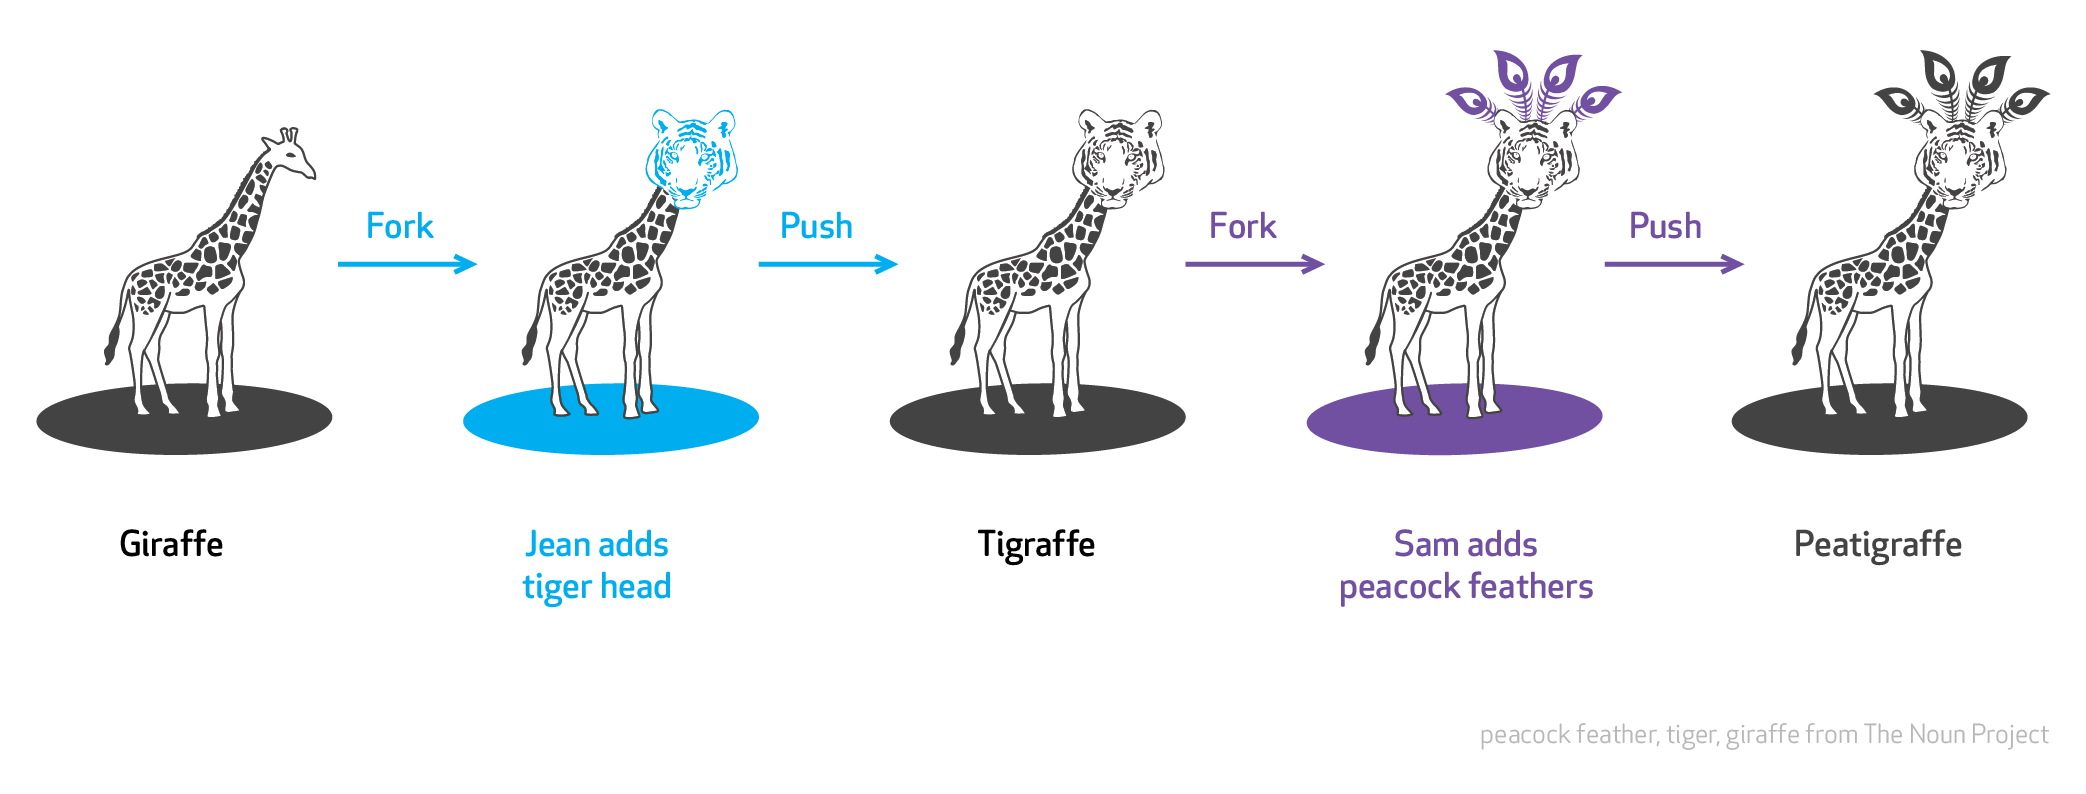
\includegraphics[width=\textwidth]{pic/git-OS.png}
\end{frame}


\begin{frame}{Social space}
\begin{itemize}
	\item \url{https://github.com/tomojitakasu/RTKLIB/issues}
	\item \url{https://gist.github.com/forked}
\end{itemize}
\end{frame}


\begin{frame}{Big guys' open source}
\centering

\includegraphics[width=.6\textwidth]{pic/Tensorflow.png}\footnote{\url{https://www.tensorflow.org/}}
\end{frame}


%%%%%%%%%%%%%%%%%%%%%%%%%%%%%%%%%%%%%%%%%%%%%%%%%%%%%%%%%%%%%%%%%%%%%%%%%%%%%%%%%%%%%%%%
\section{Reproducible research}

\begin{frame}[fragile]{Reproducible research}

\textbf{Reproducible research} is the idea that data analyses, and more generally, scientific claims, are published with their data and software code so that others may verify the findings and build upon them\footnote[frame]{Quoted after Roger Peng (Johns Hopkins University)}.

\bigskip
This means that both data and the analysis code are available allowing others to easily execute the same analysis to obtain the same results.

\end{frame}


\begin{frame}{Why?}%{Daily repetition}

\centering
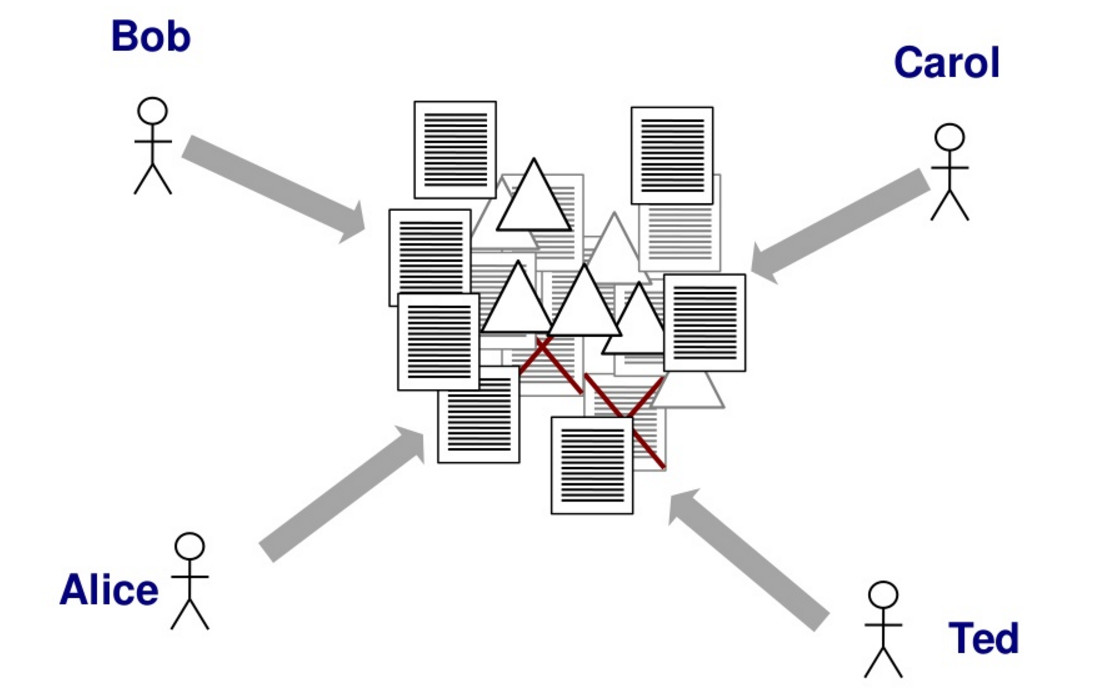
\includegraphics[width=\textwidth]{pic/disaster.jpg}\footnote{\url{http://www.slideshare.net/jomikr/quick-introduction-to-git}}

\end{frame}


\begin{frame}[fragile]{Maintaining data}

Prof Keith A. Baggerly discussed sampling errors on cancer research\footnote{Cancer Bioinformatics Workshop, Cambridge 2010 - \url{http://bit.ly/235DoBa}}. A number of research institutions The concept is very popular in computer science and engineering as well:

\begin{itemize}
	\item Stanford Exploration Project - \url{http://sepwww.stanford.edu/}
	\item Computer vision - \url{http://www.csee.wvu.edu/~xinl/}
	\item Wavelab - \url{http://finmath.stanford.edu/~wavelab/}
\end{itemize}

There is even Coursera course on the topic\footnote{\url{https://www.coursera.org/learn/reproducible-research}}.

\end{frame}


\begin{frame}[fragile]{Understanding science}


\begin{itemize}
	\item Gravitational Wave - \url{http://bit.ly/LIGO_OS}
	\item Earthquakes - \url{http://bit.ly/1MbL6C9}
	%\item Hawkers in Singapore - \url{https://rpubs.com/JoshMah/168498}
	%\item interactive plots - \url{https://plot.ly/r/}
	\item Heroes interaction - \url{http://bit.ly/1RDJ4Lv}
	\item Faces recognition - \url{http://bit.ly/1XgqjxS}
	%\item ... more at \url{http://bit.ly/1MbL6C9}
\end{itemize}

\end{frame}

%https://github.com/ipython/ipython/wiki/A-gallery-of-interesting-IPython-Notebooks
%https://www.dominodatalab.com/showcase

%%%%%%%%%%%%%%%%%%%%%%%%%%%%%%%%%%%%%%%%%%%%%%%%%%%%%%%%%%%%%%%%%%%%%%%%%%%%%%%%%%%%%%%%
\section{Wrap up}

\begin{frame}
\begin{itemize}
	\item git
	\begin{itemize}
		\item backup \& maintain your work;
		\item has application in teaching, research or learning;
		\item a social tool.
	\end{itemize}
	\item Reproducible research
	\begin{itemize}
		\item make it easy to return to the data and analyses;
		\item make it easy to share information internally \& externally;
		\item provide research scrutiny and transparency;
		\item can be great self-marketing tool.
	\end{itemize}
\end{itemize}
\end{frame}

%Final slide
\setbeamercolor{background canvas}{bg=blueBgd!60}
%\plain{
\includegraphics[width=.6\textwidth]{pic/git.png}}
\plain{Thank you}
\setbeamercolor{background canvas}{bg=blueBgd!0}

\begin{frame}
\centering

\includegraphics[height=.8\textheight]{pic/git.png}
\end{frame}


\end{document}

%http://explainxkcd.com/wiki/index.php/1597:_Git